\section{Probability Density Function (PDF) and Continuous Support}

	A non-discrete random variable $X$ is called \emph{absolutely continuous} (or simply \emph{continuous}) if its distribution function can be represented as
	\begin{align}
		 \label{eq:2.7.1}
		 F(x)=P(X \leq x)=\int_{-\infty}^{x} f(u)du, \; -\infty < x <\infty.
	\end{align}

	The function $f$ is usually called the \emph{probability density function} (or simply \emph{density function}) and must satisfy the following properties:
	\begin{enumerate}
		\item $f(x)\geq 0 $
		\item $\displaystyle \int_{-\infty}^{\infty}f(x)dx=1.$
	\end{enumerate}

	The probability that $X$ lies between two values $a$ and $b$ is given by
	\begin{align}
		\label{eq:2.7.2}
		P(a < x <b)=\int_{a}^{b}f(x)dx.
	\end{align}

	\begin{align}
		\label{eq:2.7.3}
		P(X=a)=0.
	\end{align}

Therefore, in \eqref{eq:2.7.2} we can replace any strict inequality sign $<$ with $\leq.$

	\begin{ejemplo}
		\label{exmp:2.7.1}
		\begin{enumerate}
			\item Find the constant $c$ such that the function
			\begin{align}
				f(x)=
				\begin{cases}
					cx^{2} & 0 < x < 3 \\
					0 & \texttt{otherwise}
				\end{cases}
			\end{align}
			is a probability density function. 
			\item Calculate $P(1 < X < 2).$
		\end{enumerate}
	\end{ejemplo}

	\begin{ejemplo}
	  \label{exmp:2.7.2}
	  Find the distribution function for the random variable from Example \ref{exmp:2.7.1} and use it to calculate $P(1 < x \leq 2).$
	\end{ejemplo}

	The probability that $X$ lies between $x$ and $x+\Del x$ is given by
	\begin{align}
		\label{eq:2.7.4}
		P(x \leq X \leq x+\Del x)= \int_{x}^{x+\Del x}f(u)du,
	\end{align}
	so if $\Del x \approx 0,$ we have
	\begin{align}
		\label{eq:2.7.5}
		P(x \leq X \leq x+\Del x)\approx f(x) \Del x.
	\end{align}

	We can also deduce from \eqref{eq:2.7.1}, by differentiating both sides, that
	\begin{align}
		\label{eq:2.7.6}
		\dfrac{dF(x)}{dx} = f(x)
	\end{align}
at all points where $f(x)$ is continuous. That is, the derivative of the distribution function is the density function.

	\begin{observacion}
		There are random variables that are neither discrete nor continuous. For example:
		\begin{align}
			F(x)=
			\begin{cases}
				0 & x <1 \\
				\frac{x}{2} & 1 \leq x < 2 \\
				1 & x \leq 2.
			\end{cases}
		\end{align}
	\end{observacion}

 \begin{ejemplo}
  \label{exmp:2.7.3} A random variable $X$ has density function
  \begin{align}
   f(x)=\dfrac{c}{x^{2}+1}, \; -\infty < x <\infty.
  \end{align}

  \begin{enumerate}
   \item Find the value of $c$; 
   \item find the probability that
   \begin{align}
    \dfrac{1}{3}< X^{2} <1.
   \end{align}
  \end{enumerate}
 \end{ejemplo}

 \begin{ejemplo}
  \label{exmp:2.7.4}
  Find the distribution function corresponding to the density function from Solved Problem \ref{exmp:2.7.3}.
 \end{ejemplo}

 \begin{ejemplo}
  \label{exmp:2.7.5}
  The distribution function for a random variable $X$ is
  \begin{align}
   F(x)=
   \begin{cases}
    1-e^{-2x} & x\geq 0 \\
    0 & x <0
   \end{cases}
  \end{align}

  Find
  \begin{enumerate}
   \item the density function;
   \item the probability that $X>2$;
   \item the probability that $-3 < X \leq 4.$
  \end{enumerate}
 \end{ejemplo}

\section{Cumulative Distribution Function (CDF), Continuous Case}
\subsection{Graphical Interpretation}

	The distribution function $F(x)=P(X\leq x)$ is monotonically increasing from $0$ to $1...$
	\begin{figure}
	\centering
	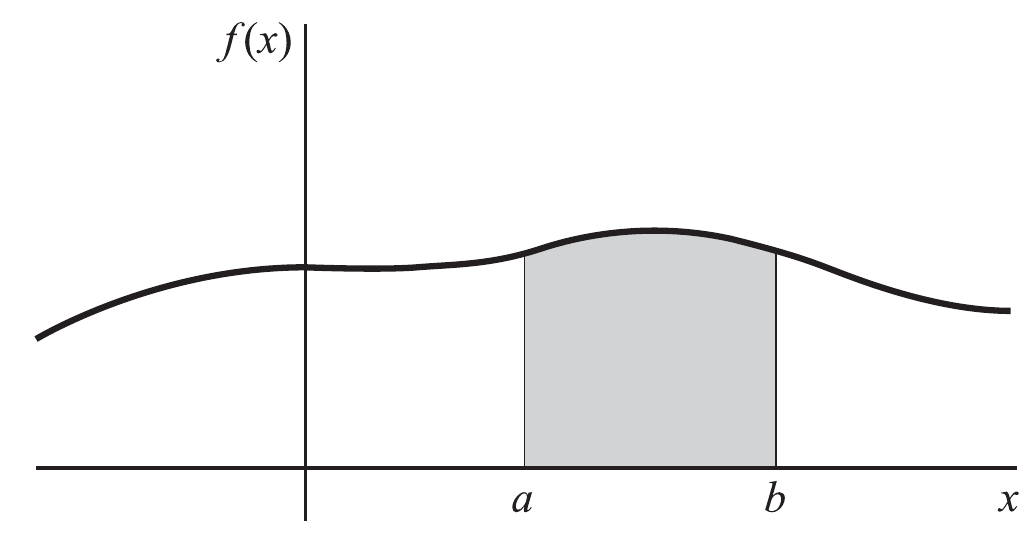
\includegraphics[height=5cm,keepaspectratio=true]{./pe/pands0202.png}
	% pands0202.png: 0x0 pixel, 300dpi, 0.00x0.00 cm, bb=
\end{figure}

  ...and the area under the density curve is equal to $1.$
  \begin{figure}
	\centering
	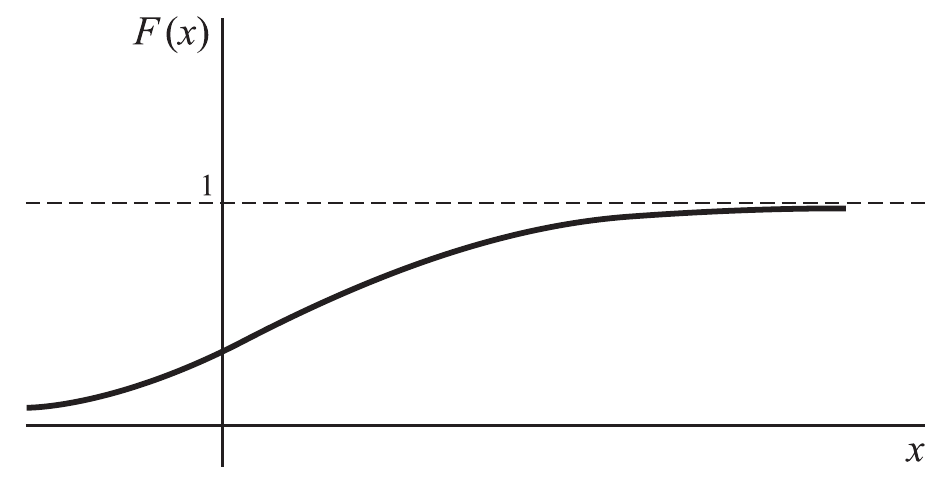
\includegraphics[height=5cm,keepaspectratio=true]{./pe/pands0203.png}
	% pands0203.png: 0x0 pixel, 300dpi, 0.00x0.00 cm, bb=
\end{figure}

\subsection{Joint Probability Distribution}

	The preceding ideas are easily generalized to two or more variables.

{Discrete case}
	If $X$ and $Y$ are both discrete random variables, we define the \emph{joint probability function} of $X$ and $Y$ by
	\begin{align}
	\label{eq:2.7.7}
		P(X=x, Y=y)=f(x,y)
	\end{align}
 where
\begin{enumerate}
	\item $f(x,y)\geq 0;$
	\item $\sum_{k}\sum_{y}f(x,y)=1.$
\end{enumerate}

	Suppose that $X$ takes only one of the $m$ values $x_{1},...,x_{m},$ while $Y$ takes only one of the $n$ values $y_{1},...,y_{n}.$

	Then the probability of the event $X=x_{j}, Y=y_{k}$ is given by
	\begin{align}
	\label{eq:2.7.8}
		P(X=x_{j}, Y=y_{k})=f(x_{j},y_{k})
	\end{align}

	A joint probability function for $X$ and $Y$ can be represented by a \emph{joint probability table} such as the following:
	\begin{figure}
	\centering
		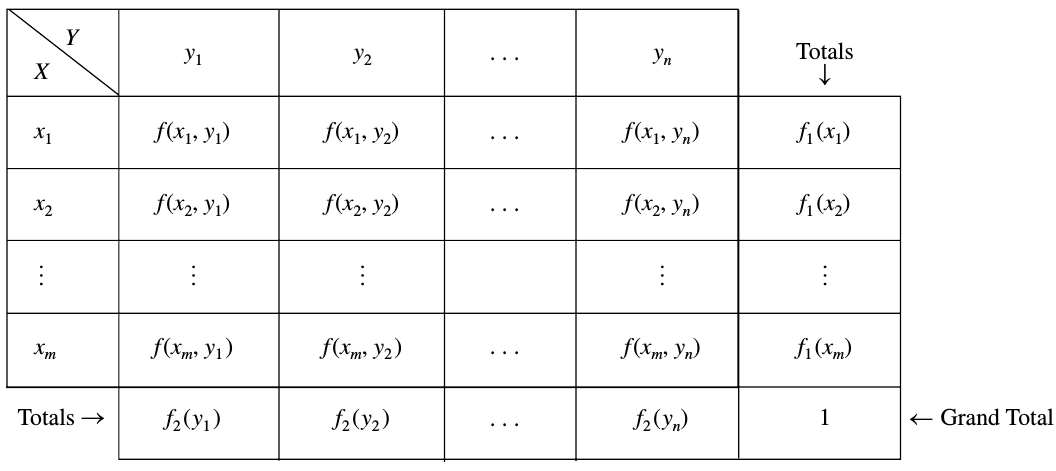
\includegraphics[height=5cm,keepaspectratio=true]{./pe/tab0203.png}
		% tab0203.png: 0x0 pixel, 300dpi, 0.00x0.00 cm, bb=
		\label{tab:2.7.1}
	\end{figure}

	The probability of $X=x_{j}$ is obtained as follows:
	\begin{align}
	\label{eq:2.7.9}
		P(X=x_{j})=f_{X}(x_{j})=\sum_{k=1}^{n}f(x_{j},y_{k}).
	\end{align}

	Similarly, the probability of $Y=y_{k}$ is obtained as follows:
	\begin{align}
	\label{eq:2.7.10}
		P(Y=y_{k})=f_{Y}(y_{k})=\sum_{j=1}^{m}f(x_{j},y_{k}).
	\end{align}

  	We refer to $f_{X}(x)$ and $f_{Y}(y)$ as the \emph{marginal probability functions} of $X$ and $Y$, respectively.

	Note that
	\begin{align}
	\label{eq:2.7.11}
		\sum_{j=1}^{m}f_{X}(x_{j})=1,
		\sum_{k=1}^{n}f_{Y}(y_{k})=1,
	\end{align}
	which can be rewritten as
	\begin{align}
		\label{eq:2.7.12}
		\sum_{j=1}^{m}\sum_{k=1}^{n}f(x_{j},y_{k})=1.
	\end{align}

	The \emph{joint distribution function} is defined by
	\begin{align}
	\label{eq:2.7.13}
		F(x,y)=P(X\leq x, Y\leq y)
		=\sum_{u\leq x}\sum_{v\leq y}f(u,v)
	\end{align}

{Continuous case}
	The case where both variables are continuous is obtained analogously by replacing sums with integrals.

	The \emph{joint probability function} (or more commonly \emph{joint density function}) of $X$ and $Y$ is defined such that:
	\begin{enumerate}
		\item $f(x,y)\geq 0;$
		\item $\displaystyle \int_{-\infty}^{\infty}\int_{-\infty}^{\infty}
		f(x,y) dxdy=1.$
	\end{enumerate}

	Graphically, $z=f(x,y)$ represents a \emph{probability surface}
\begin{figure}
	\centering
		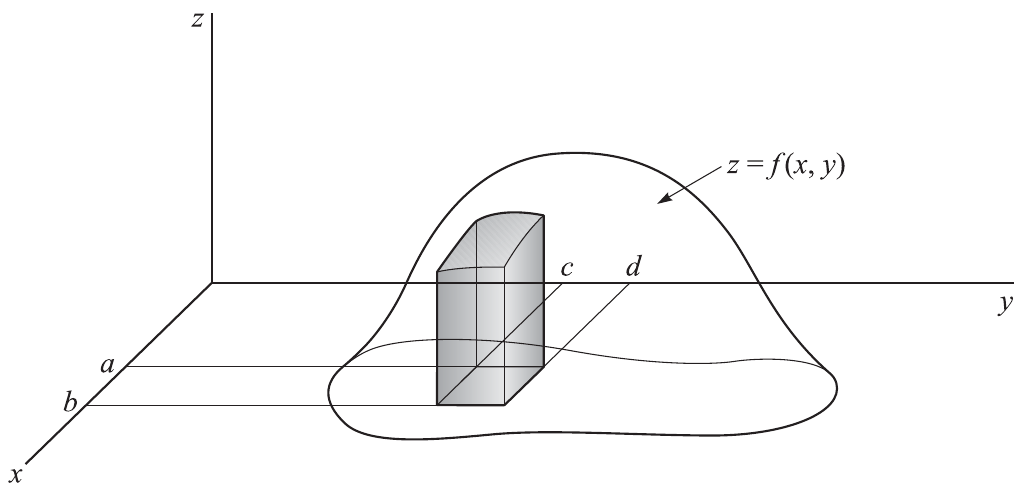
\includegraphics[height=3cm,keepaspectratio=true]{./pe/pands0204.png}
		% pands0204.png: 0x0 pixel, 300dpi, 0.00x0.00 cm, bb=
		\label{fig:2.7.1}
	\end{figure}
such that the volume under the surface is equal to $1.$

	\begin{align}
		\label{eq:2.7.14}
		P(a<X<b,c<Y<d)=\int_{a}^{b}\int_{c}^{d}f(x,y)dydx.
	\end{align}

	To each event $A$ there corresponds a region $\mathcal{R}_{A}$ of the $xy$-plane such that
	\begin{align}
	  \label{eq:2.7.15}
		P(A)=\iint_{\mathcal{R}_{A}}f(x,y)dxdy.
	\end{align}

	The \emph{joint distribution function} of $X$ and $Y$ in this case is defined by
	\begin{align}
		\label{eq:2.7.16}
	F(x,y)=P(X\leq x, Y\leq y)=
	\int_{-\infty}^{x} \int_{-\infty}^{y} f(u,v)dvdu.
	\end{align}

	It follows that
	\begin{align}
	 \dfrac{\partial^{2}F}{\partial x \partial y}=
	 f(x,y)  \label{eq:2.7.17} \\
	  	 P(X\leq x)=F_{X}(x)=\int_{-\infty}^{x}\int_{-\infty}^{\infty} f(u,v)dvdu \label{eq:2.7.18} \\
	 	 P(Y\leq y)=F_{Y}(y)=\int_{-\infty}^{\infty}\int_{-\infty}^{y} f(u,v)dvdu \label{eq:2.7.19}
	\end{align}

  We say that $F_{X}(x)$ and $F_{Y}(y)$ are the \emph{marginal distribution functions}, or simply \emph{distribution functions}, of $X$ and $Y$, respectively.

  The derivatives of \eqref{eq:2.7.18} and \eqref{eq:2.7.19} with respect to $x$ and $y$ are called the \emph{marginal density functions}, or simply the \emph{density functions}, of $X$ and $Y$ and are given by
  \begin{align}
  \label{eq:2.7.20}
  \displaystyle
   f_{X}(x)=\int_{-\infty}^{\infty}f(x,v)dv, \;
   f_{Y}(y)=\int_{-\infty}^{\infty}f(u,y)du.
  \end{align}

 \subsection{Independent Random Variables}

  Suppose $X$ and $Y$ are discrete random variables. If the events $X=x$ and $Y=y$ are independent events for all $x,y,$ then we say that $X,Y$ are independent random variables.

  In such a case,
  \begin{align}
   \label{eq:2.7.21}
   P(X=x,Y=y)=P(X=x)P(Y=y),
  \end{align}
or equivalently
\begin{align}
 f(x,y)=f_{X}(x)f_{Y}(y).
\end{align}

  Conversely, if for all $x,y$ the joint probability function $f(x,y)$ can be expressed as the product of the marginal probability functions $f_{X}(x)f_{Y}(y),$ then $X,Y$ are independent.

  If they cannot be expressed in this way, then $X,Y$ are dependent.

  If $X,Y$ are continuous random variables, we say they are \emph{independent} if the events $X\leq x$ and $Y\leq y$ are independent for all $x,y.$

  In such a case, we write
  \begin{align}
   \label{eq:2.7.22}
   P(X\leq x, Y \leq y)=P(X\leq x)P(Y\leq y)
  \end{align}
  or equivalently
  \begin{align}
   F(x,y)=F_{X}(x)F_{Y}(y)
  \end{align}
  where $F_{X}(x)$ and $F_{Y}(y)$ are the marginal distribution functions of $X$ and $Y$, respectively.

  Conversely, if for all $x,y$ the joint distribution function $F(x,y)$ can be expressed as the product of the marginal distribution functions $F_{X}(x)F_{Y}(y),$ then $X,Y$ are independent.
  
  If they cannot be expressed in this way, then $X,Y$ are dependent.

  For independent continuous random variables, it is also true that the joint density function $f(x,y)$ is the product of the functions $f_{X}(x)f_{Y}(y)$, which are the marginal density functions of $X$ and $Y$, respectively.

 \begin{ejemplo}
  \label{exmp:2.7.6}
  The joint probability function of two discrete variables $X,Y$ is given by
  \begin{align}
   f(x,y)=
   \begin{cases}
    c(2x+y) & 0\leq x \leq 2, \; 0 \leq y \leq 3 \\
    0 & \texttt{otherwise}.
   \end{cases}
  \end{align}
  \begin{enumerate}
   \item Find the value of the constant $c;$
   \item find $P(X=2,Y=1);$
   \item find $P(X\geq 1, Y\leq 2).$
  \end{enumerate}
 \end{ejemplo}

 \begin{figure}
 \centering
	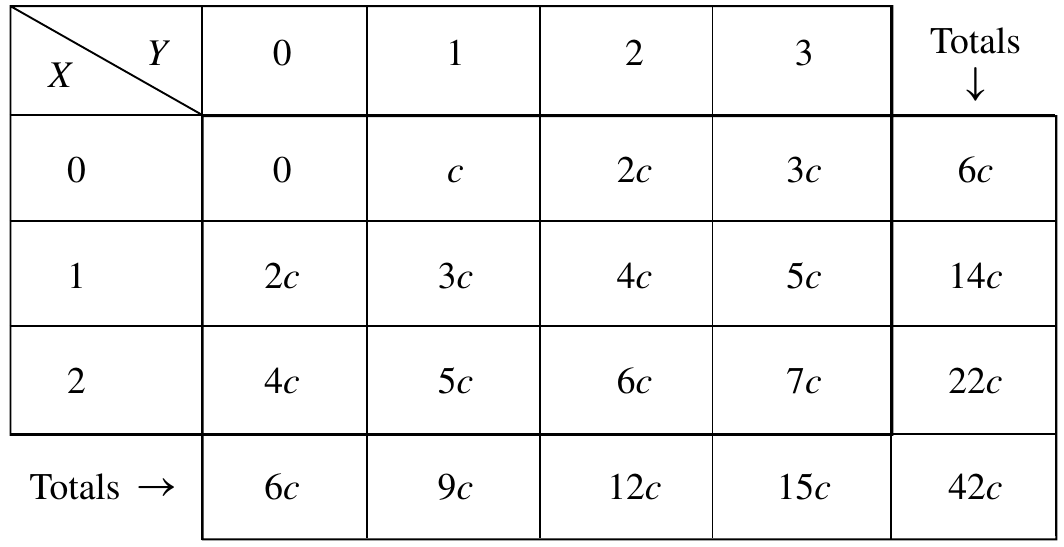
\includegraphics[width=10cm,keepaspectratio=true]{./pe/tab0206.png}
	% tab0206.png: 0x0 pixel, 300dpi, 0.00x0.00 cm, bb=
	\label{tab:2.7.2}
\end{figure}

\begin{ejemplo}
  \label{exmp:2.7.7}
  Find the marginal probability functions for $X$ and $Y$ in Solved Problem \ref{exmp:2.7.6}.
\end{ejemplo}

\begin{ejemplo}
  \label{exmp:2.7.8}
  Show that the random variables of Solved Problem \ref{exmp:2.7.6} are dependent.
\end{ejemplo}

\begin{ejemplo}
  \label{exmp:2.7.9}
  The joint density function of two continuous random variables $X$ and $Y$ is
  \begin{align}
   f(x,y)=
   \begin{cases}
    cxy & 0<x<4, \; 1<y<5\\
    0 & \texttt{otherwise}.
   \end{cases}
  \end{align}
 \end{ejemplo}
\begin{enumerate}
 \item Find the value of $c$;
 \item find $P(1<X<2,2<Y<3)$;
 \item find $P(X\geq 3, Y\leq 2)$.
\end{enumerate}

\begin{ejemplo}
  \label{exmp:2.7.10}
  Find the marginal probability density functions of the random variables $X,Y$ from Solved Problem \ref{exmp:2.7.9}.
\end{ejemplo}

\begin{ejemplo}
  \label{exmp:2.7.11}
  Find the joint distribution function for the random variables from Solved Problem \ref{exmp:2.7.9}.
\end{ejemplo}

 \begin{center}
 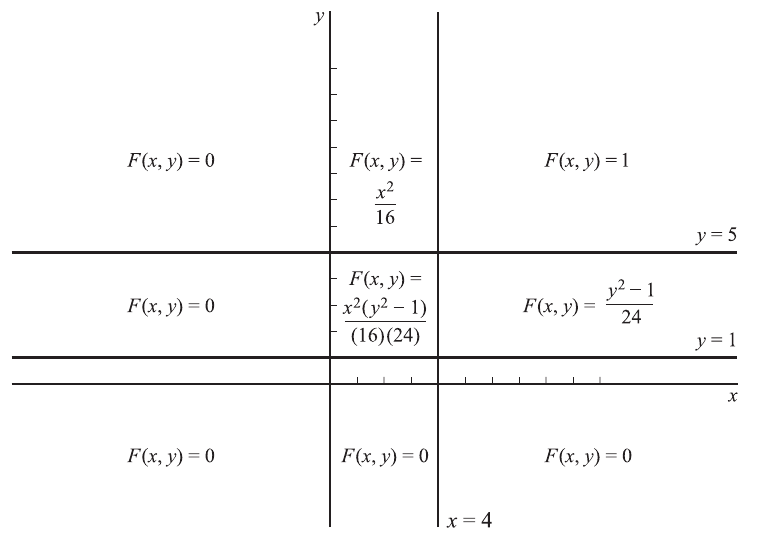
\includegraphics[width=10cm,keepaspectratio=true]{./pe/pands0209.png}
 % pands0209.png: 0x0 pixel, 300dpi, 0.00x0.00 cm, bb=
\end{center}

\begin{ejemplo}
  \label{exmp:2.7.12}
  In Solved Problem \ref{exmp:2.7.9}, find $P(X+Y<3)$.
\end{ejemplo}

 \begin{center}
 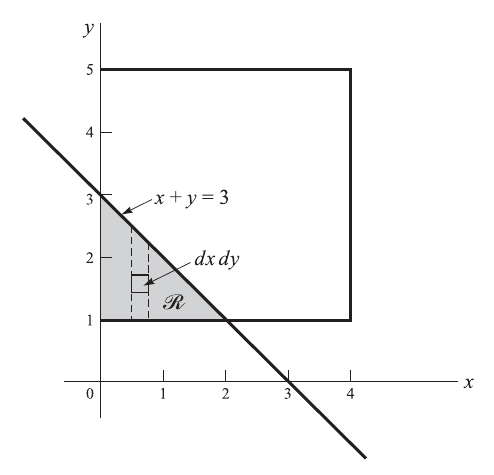
\includegraphics[height=8cm,keepaspectratio=true]{./pe/pands0210.png}
 % pands0210.png: 0x0 pixel, 300dpi, 0.00x0.00 cm, bb=
\end{center}

 \subsection{Conditional Distribution}

 We already know that if $P(A)>0,$
 \begin{align}
  \label{eq:2.7.23}
  P(B|A)=\dfrac{P(A\cap B)}{P(A)}.
 \end{align}

 If $X,Y$ are discrete random variables and we consider the events $A=\set{X=x}, \; B=\set{Y=y},$ then \eqref{eq:2.7.23} becomes
 \begin{align}
  \label{eq:2.7.24}
  P(Y=y|X=x)=
  \begin{cases}
   \dfrac{f(x,y)}{f_{X}(x)} & 0 < f_{X}(x)  \\
   0 & \texttt{otherwise}
  \end{cases}
 \end{align}
 where $f(x,y)=P(X=x,Y=y)$ is the joint probability function, while $f_{X}(x)$ is the marginal probability function for $X.$

 We define the \emph{conditional probability function of $Y$ given $X$} as
 \begin{align}
  \label{eq:2.7.25}
  f(y|x)=
  \begin{cases}
   \dfrac{f(x,y)}{f_{X}(x)} & 0 < f_{X}(x)  \\
   0 & \texttt{otherwise}
  \end{cases}
 \end{align}

 Similarly, we define the \emph{conditional probability function of $X$ given $Y$} as
 \begin{align}
  \label{eq:2.7.26}
  f(x|y)=
  \begin{cases}
   \dfrac{f(x,y)}{f_{Y}(y)} & 0 < f_{Y}(y)  \\
   0 & \texttt{otherwise}
  \end{cases}
 \end{align}

 These ideas are easily extended to the case where $X,Y$ are continuous random variables.

 For example, the \emph{conditional density function of $Y$ given $X$} is
 \begin{align}
  \label{eq:2.7.27}
  f(y|x)=
    \begin{cases}
   \dfrac{f(x,y)}{f_{X}(x)} & 0 < f_{X}(x)  \\
   0 & \texttt{otherwise}
  \end{cases}
 \end{align}
 where $f(x,y)$ is the joint density function of $X$ and $Y$ and $f_{X}(x)$ is the marginal density function of $X.$

 Using \eqref{eq:2.7.27} we can, for instance, find that the probability that $Y$ lies between $c$ and $d$ given that $X=x$ is
 \begin{align}
  \label{eq:2.7.28}P(c<Y<d|X=x)=
  \int_{c}^{d}f(y|x)dy.
 \end{align}

 \begin{ejemplo}
  \label{exmp:2.7.13}
  For the distribution of Solved Problem \ref{exmp:2.7.6}, find
  \begin{enumerate}
   \item $f(y|2)$; and
   \item $P(Y=1|X=2)$
  \end{enumerate}
 \end{ejemplo}

\begin{ejemplo}
 \label{exmp:2.7.14}
  If $X$ and $Y$ have joint density function
 \begin{align}
  f(x,y)=
  \begin{cases}
   \frac{3}{4}+xy & 0<x<1, \; 0<y<1 \\
   0 & \texttt{otherwise},
  \end{cases}
 \end{align}
find
\begin{enumerate}
 \item $f(y|x)$; 
 \item $P(Y>\frac{1}{2}| X = \frac{1}{2} )$.
\end{enumerate}
\end{ejemplo}

 \begin{ejemplo}
  \label{exmp:2.7.15}
  The joint density function of the random variables $X$ and $Y$ is given by
  \begin{align}
   f(x,y)=
   \begin{cases}
    8xy & 0\leq x \leq 1, 0\leq y \leq x \\
    0 & \texttt{otherwise}.
   \end{cases}
  \end{align}
Find
\begin{enumerate}
 \item the marginal density of $X$; 
 \item the marginal density of $Y$; 
 \item the conditional density of $X$; 
 \item the conditional density of $Y$.
\end{enumerate}
 \end{ejemplo}

 \begin{center}
 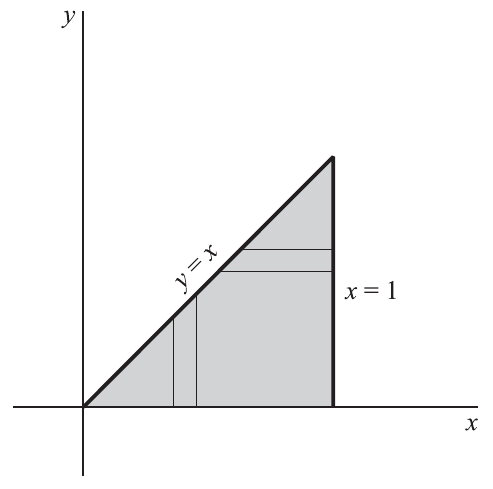
\includegraphics[height=7cm,keepaspectratio=true]{./pe/pands0217.png}
 % pands0217.png: 0x0 pixel, 300dpi, 0.00x0.00 cm, bb=
\end{center}

 \begin{ejemplo}
  \label{exmp:2.7.16}
  Determine whether the random variables from Solved Problem \ref{exmp:2.7.15} are independent.
 \end{ejemplo}
